% Options for packages loaded elsewhere
\PassOptionsToPackage{unicode}{hyperref}
\PassOptionsToPackage{hyphens}{url}
%
\documentclass[
  10pt,
]{article}
\usepackage{amsmath,amssymb}
\usepackage{iftex}
\ifPDFTeX
  \usepackage[T1]{fontenc}
  \usepackage[utf8]{inputenc}
  \usepackage{textcomp} % provide euro and other symbols
\else % if luatex or xetex
  \usepackage{unicode-math} % this also loads fontspec
  \defaultfontfeatures{Scale=MatchLowercase}
  \defaultfontfeatures[\rmfamily]{Ligatures=TeX,Scale=1}
\fi
\usepackage{lmodern}
\ifPDFTeX\else
  % xetex/luatex font selection
\fi
% Use upquote if available, for straight quotes in verbatim environments
\IfFileExists{upquote.sty}{\usepackage{upquote}}{}
\IfFileExists{microtype.sty}{% use microtype if available
  \usepackage[]{microtype}
  \UseMicrotypeSet[protrusion]{basicmath} % disable protrusion for tt fonts
}{}
\makeatletter
\@ifundefined{KOMAClassName}{% if non-KOMA class
  \IfFileExists{parskip.sty}{%
    \usepackage{parskip}
  }{% else
    \setlength{\parindent}{0pt}
    \setlength{\parskip}{6pt plus 2pt minus 1pt}}
}{% if KOMA class
  \KOMAoptions{parskip=half}}
\makeatother
\usepackage{xcolor}
\usepackage[margin=0.7in]{geometry}
\usepackage{color}
\usepackage{fancyvrb}
\newcommand{\VerbBar}{|}
\newcommand{\VERB}{\Verb[commandchars=\\\{\}]}
\DefineVerbatimEnvironment{Highlighting}{Verbatim}{commandchars=\\\{\}}
% Add ',fontsize=\small' for more characters per line
\newenvironment{Shaded}{}{}
\newcommand{\AlertTok}[1]{\textcolor[rgb]{1.00,0.00,0.00}{\textbf{#1}}}
\newcommand{\AnnotationTok}[1]{\textcolor[rgb]{0.38,0.63,0.69}{\textbf{\textit{#1}}}}
\newcommand{\AttributeTok}[1]{\textcolor[rgb]{0.49,0.56,0.16}{#1}}
\newcommand{\BaseNTok}[1]{\textcolor[rgb]{0.25,0.63,0.44}{#1}}
\newcommand{\BuiltInTok}[1]{\textcolor[rgb]{0.00,0.50,0.00}{#1}}
\newcommand{\CharTok}[1]{\textcolor[rgb]{0.25,0.44,0.63}{#1}}
\newcommand{\CommentTok}[1]{\textcolor[rgb]{0.38,0.63,0.69}{\textit{#1}}}
\newcommand{\CommentVarTok}[1]{\textcolor[rgb]{0.38,0.63,0.69}{\textbf{\textit{#1}}}}
\newcommand{\ConstantTok}[1]{\textcolor[rgb]{0.53,0.00,0.00}{#1}}
\newcommand{\ControlFlowTok}[1]{\textcolor[rgb]{0.00,0.44,0.13}{\textbf{#1}}}
\newcommand{\DataTypeTok}[1]{\textcolor[rgb]{0.56,0.13,0.00}{#1}}
\newcommand{\DecValTok}[1]{\textcolor[rgb]{0.25,0.63,0.44}{#1}}
\newcommand{\DocumentationTok}[1]{\textcolor[rgb]{0.73,0.13,0.13}{\textit{#1}}}
\newcommand{\ErrorTok}[1]{\textcolor[rgb]{1.00,0.00,0.00}{\textbf{#1}}}
\newcommand{\ExtensionTok}[1]{#1}
\newcommand{\FloatTok}[1]{\textcolor[rgb]{0.25,0.63,0.44}{#1}}
\newcommand{\FunctionTok}[1]{\textcolor[rgb]{0.02,0.16,0.49}{#1}}
\newcommand{\ImportTok}[1]{\textcolor[rgb]{0.00,0.50,0.00}{\textbf{#1}}}
\newcommand{\InformationTok}[1]{\textcolor[rgb]{0.38,0.63,0.69}{\textbf{\textit{#1}}}}
\newcommand{\KeywordTok}[1]{\textcolor[rgb]{0.00,0.44,0.13}{\textbf{#1}}}
\newcommand{\NormalTok}[1]{#1}
\newcommand{\OperatorTok}[1]{\textcolor[rgb]{0.40,0.40,0.40}{#1}}
\newcommand{\OtherTok}[1]{\textcolor[rgb]{0.00,0.44,0.13}{#1}}
\newcommand{\PreprocessorTok}[1]{\textcolor[rgb]{0.74,0.48,0.00}{#1}}
\newcommand{\RegionMarkerTok}[1]{#1}
\newcommand{\SpecialCharTok}[1]{\textcolor[rgb]{0.25,0.44,0.63}{#1}}
\newcommand{\SpecialStringTok}[1]{\textcolor[rgb]{0.73,0.40,0.53}{#1}}
\newcommand{\StringTok}[1]{\textcolor[rgb]{0.25,0.44,0.63}{#1}}
\newcommand{\VariableTok}[1]{\textcolor[rgb]{0.10,0.09,0.49}{#1}}
\newcommand{\VerbatimStringTok}[1]{\textcolor[rgb]{0.25,0.44,0.63}{#1}}
\newcommand{\WarningTok}[1]{\textcolor[rgb]{0.38,0.63,0.69}{\textbf{\textit{#1}}}}
\usepackage{longtable,booktabs,array}
\usepackage{calc} % for calculating minipage widths
% Correct order of tables after \paragraph or \subparagraph
\usepackage{etoolbox}
\makeatletter
\patchcmd\longtable{\par}{\if@noskipsec\mbox{}\fi\par}{}{}
\makeatother
% Allow footnotes in longtable head/foot
\IfFileExists{footnotehyper.sty}{\usepackage{footnotehyper}}{\usepackage{footnote}}
\makesavenoteenv{longtable}
\usepackage{graphicx}
\makeatletter
\def\maxwidth{\ifdim\Gin@nat@width>\linewidth\linewidth\else\Gin@nat@width\fi}
\def\maxheight{\ifdim\Gin@nat@height>\textheight\textheight\else\Gin@nat@height\fi}
\makeatother
% Scale images if necessary, so that they will not overflow the page
% margins by default, and it is still possible to overwrite the defaults
% using explicit options in \includegraphics[width, height, ...]{}
\setkeys{Gin}{width=\maxwidth,height=\maxheight,keepaspectratio}
% Set default figure placement to htbp
\makeatletter
\def\fps@figure{htbp}
\makeatother
\setlength{\emergencystretch}{3em} % prevent overfull lines
\providecommand{\tightlist}{%
  \setlength{\itemsep}{0pt}\setlength{\parskip}{0pt}}
\setcounter{secnumdepth}{-\maxdimen} % remove section numbering
\ifLuaTeX
  \usepackage{selnolig}  % disable illegal ligatures
\fi
\usepackage{bookmark}
\IfFileExists{xurl.sty}{\usepackage{xurl}}{} % add URL line breaks if available
\urlstyle{same}
\hypersetup{
  hidelinks,
  pdfcreator={LaTeX via pandoc}}

\author{}
\date{}

\begin{document}

\section{Elliptic-curve surface tools ---
2026-10-11}\label{elliptic-curve-surface-tools-2026-10-11}

The integration adds three native Rust tools to both
\path|aburan28/crypto| and \path|aburan28/cryptanalysis|, under
\href{../../tools/ecdlp-surfaces/README.md}{\path|tools/ecdlp-surfaces|}.
They enumerate a bounded family of surfaces, check the group law on the
embedded curve, and filter supplied abelian-surface Frobenius
polynomials. They support point arithmetic over prime fields
\path|3 < p <= 10,000|.

The \href{PROTOCOL.md}{protocol} fixes the inputs and acceptance checks.
This is tooling and correctness evidence, with no timing comparison, new
IC candidate, catalog promotion, or destination-solver advantage. The
\href{report.pdf}{PDF}, \href{transfer.dot}{diagram source},
\href{transfer.svg}{diagram}, and \href{counts.svg}{census graphic}
accompany the report. Run \path|make -C docs/ecdlp-surfaces| to rebuild
it with Graphviz, Pandoc, pdfLaTeX, and PyMuPDF. Python here renders the
recorded graphic only.

\subsection{Exact input and identity}\label{exact-input-and-identity}

The public fixture is \path|y^2 = x^3 + x + 46| over F101, with 109
rational points, prime subgroup order 109, cofactor 1, generator
\path|P=(2,37)|, and known-answer point \path|Q=(64,19)=37P|. The origin
is the point at infinity.

Its complete field/model/subgroup metadata is in
\href{evidence/curve_record.json}{\path|evidence/curve_record.json|}:

\begin{Shaded}
\begin{Highlighting}[]
\NormalTok{EC1P7Cfph1bb53caf9319}
\NormalTok{urn:ec{-}record:1:sha256:1bb53caf931906365143bc019d9e52ffe8e4173cd4565cecd3fe832867cb6eee}
\end{Highlighting}
\end{Shaded}

Both repositories carry identical metadata, following
\href{../curve-identities.md}{\path|docs/curve-identities.md|}. This
identifies the fixture, including its field encoding and generator; it
is not an isogeny-route ID or an IC measurement ID.

\subsection{Construction and verified
results}\label{construction-and-verified-results}

The embedding sends \path|(x,y)| to \path|[1:x:y:x^2]| and the origin to
\path|[0:0:0:1]|. Its image is the intersection of \path|Q1=WZ-X^2| and
\path|Q2=Y^2-XZ-aWX-bW^2|. Every finite member \path|Q2+lambda*Q1=0|
contains the image. Substitution and the matrix determinant have native
identity certificates:

\begin{longtable}[]{@{}
  >{\raggedright\arraybackslash}p{(\columnwidth - 4\tabcolsep) * \real{0.3333}}
  >{\raggedright\arraybackslash}p{(\columnwidth - 4\tabcolsep) * \real{0.3333}}
  >{\raggedright\arraybackslash}p{(\columnwidth - 4\tabcolsep) * \real{0.3333}}@{}}
\toprule\noalign{}
\begin{minipage}[b]{\linewidth}\raggedright
Identity
\end{minipage} & \begin{minipage}[b]{\linewidth}\raggedright
Certificate
\end{minipage} & \begin{minipage}[b]{\linewidth}\raggedright
Verification
\end{minipage} \\
\midrule\noalign{}
\endhead
\bottomrule\noalign{}
\endlastfoot
Substitution into the quadric pencil &
\href{evidence/embedding_identity.json}{IDC1h72074ababc49d184} & Exact
integer-coefficient expansion and 32+32 point checks \\
\path|det(2M)=4(lambda^3+a*lambda+b)| &
\href{evidence/quadric_determinant.json}{IDC1h6e9fc67ebca6f151} & Exact
integer-coefficient expansion and 32+32 point checks \\
\end{longtable}

The \href{certificates/README.md}{native generator} replays the
certificates and rejects a false identity or corrupted digest. The
certificate schema evaluates over \path|2^61-1|; the separate
coefficient expansion checks these integer identities. Checks used one
Linux x86-64 host, not a second-host verifier. \path|proof| remains
null; no formal-prover artifact is claimed. See the
\href{evidence/identity_replay.json}{replay receipt}.

Since 2 is invertible, \path|det(M)=(lambda^3+a*lambda+b)/4|. Smoothness
is exactly nonvanishing of that value. A smooth member has the displayed
rational origin and is split over the source field precisely when the
determinant is a square. The
\href{../../tools/ecdlp-surfaces/examples/surface_candidates.json}{native
census} enumerates all 101 finite parameters: 101 smooth members and 54
split members. Thus 47 smooth members are nonsplit, derived as
\path|101-54|. The parameter at infinity is \path|Q1|, a singular
quadric, and is outside that finite census.

\begin{figure}
\centering
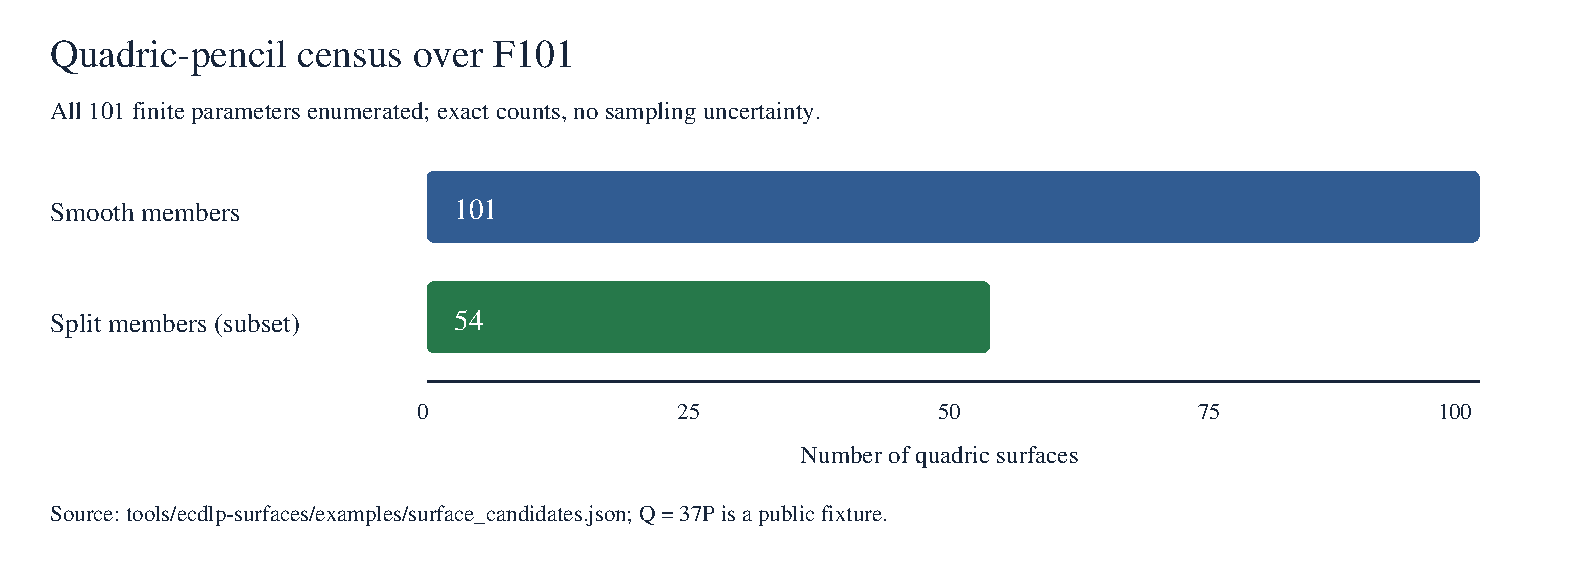
\includegraphics{counts.pdf}
\caption{Exact counts from the native census}
\end{figure}

The
\href{../../tools/ecdlp-surfaces/examples/transfer_certificate.json}{transfer
fixture} checks actual membership in the cyclic subgroup, projective
round trips, order preservation, and the public scalar witness. The law
is \path|encode(decode(U)+decode(V))| on the curve image. Points lying
only on a containing surface are rejected. Rank-two rational torsion is
a negative control: \path|rQ=O| alone does not establish that \path|Q|
belongs to \path|<P>|.

The product \path|E x E| supplies an ambient abelian-surface group law,
with the injective map \path|P -> (P,O)|. It is a trivial transfer and
supplies no solver advantage. The diagram distinguishes it from
containment in a quadric.

\begin{figure}
\centering
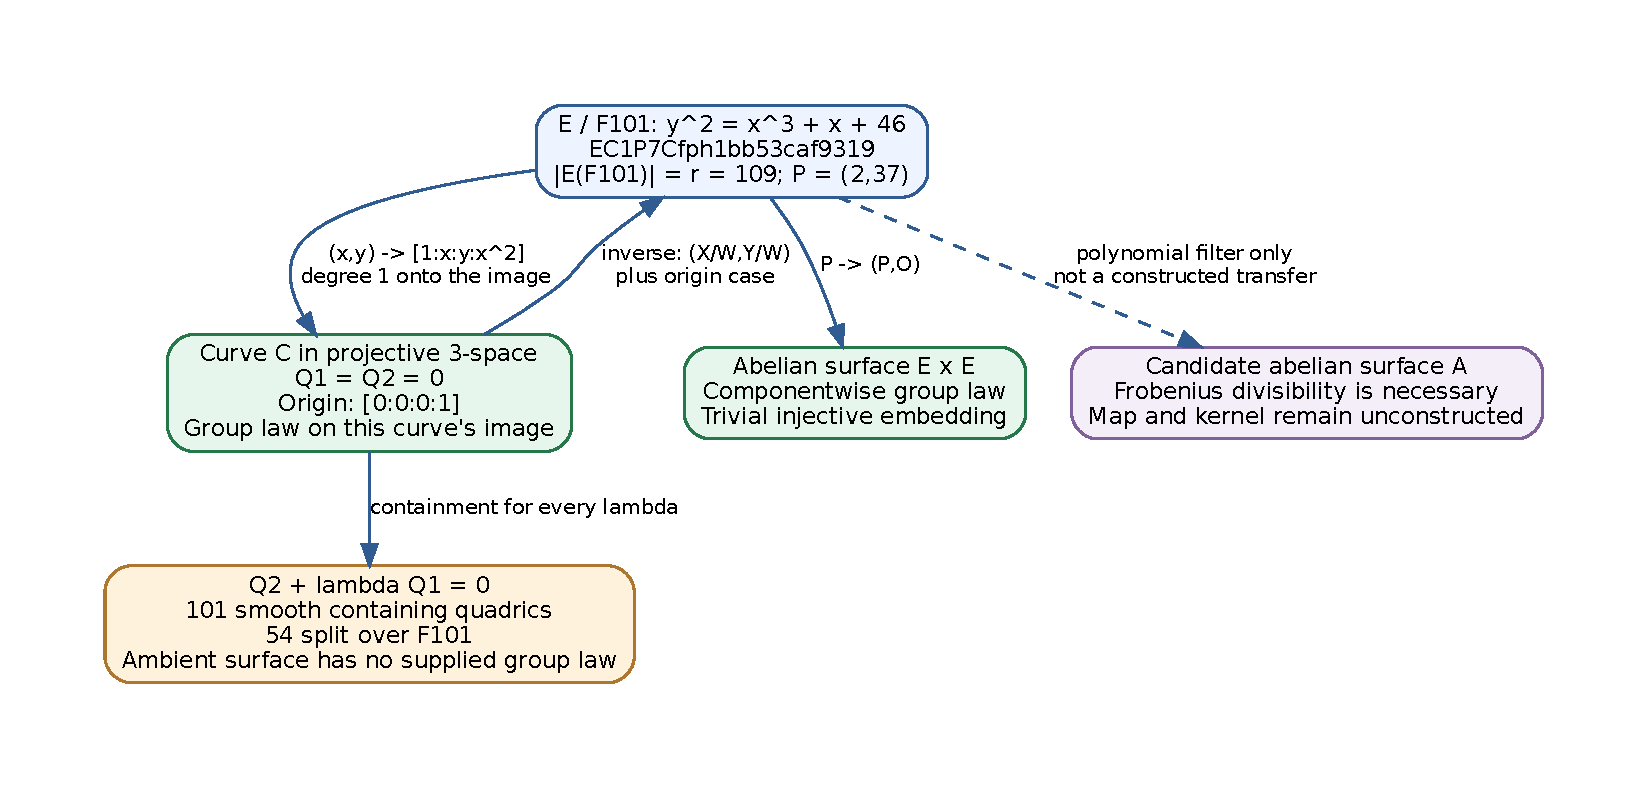
\includegraphics{transfer.pdf}
\caption{Containment, transported law, and the conditional surface
filter}
\end{figure}

\subsection{Necessary filter and negative
findings}\label{necessary-filter-and-negative-findings}

For an actual abelian surface over the same finite field, a nonzero
algebraic homomorphism from the source elliptic curve requires its
Frobenius polynomial as a factor. The supplied-polynomial filter checks
divisibility, reciprocal conditions, and the elliptic quotient's Hasse
bound. The source polynomial is \path|T^2+7T+101|; its square passes the
\href{../../tools/ecdlp-surfaces/examples/frobenius_result.json}{compatible
example}. The polynomial \path|(T^2+101)^2| fails the
\href{evidence/incompatible_frobenius.json}{incompatible control}.

Passing this necessary filter does not establish existence of a variety,
construct a homomorphism, determine its kernel, or certify subgroup
transfer. Prime-power validity and all Honda-Tate existence conditions
are unimplemented. The current checker uses small-subgroup enumeration
for membership; it is not a scalable transfer verifier or an ECDLP
accelerator. Arbitrary new surface constructions, their maps and
kernels, and a faster destination solver remain unimplemented. A bounded
pencil search is not a search over all surfaces.

\subsection{Validation and delivery
status}\label{validation-and-delivery-status}

\path|tools/ecdlp-surfaces/check.sh| passed separately in both
checkouts: formatting, 13 release tests, Clippy with warnings denied,
all three binaries, byte-identical example replay, and rejection of an
incorrect witness and a composite modulus. The certificate package
passed 3 release tests, including standard hash vectors, false-identity
refusal, and digest-tampering rejection; its formatting and Clippy also
passed. Reproduction commands are in the crate and certificate READMEs.
The \href{evidence/integration_checks.json}{verification record} retains
exact commands, repository revisions, and scope.

The required \path|crypto| root-library check was attempted and failed
on an existing syntax error in
\path|src/cryptanalysis/koblitz_factor_base_search.rs:1608|, ending with
an unexpected closing delimiter at line 1854. That file is unchanged by
this integration. The
\href{evidence/crypto_library_check.txt}{diagnostic excerpt} records the
failed gate; the root library is not reported as passing. A bounded
attempt to remove the stray line exposed another malformed function in
\path|koblitz_index_calculus.rs|; that attempted repair was reverted.
Both larger library source files remain unchanged, and both diagnostics
are retained. Conductor is unavailable (\path|conductor check| exits
127). GitHub authentication returns HTTP 401, preventing branch
publication and ready-for-review PR creation. Local commits and patches
are the available delivery while that access is blocked.

\begin{longtable}[]{@{}
  >{\raggedright\arraybackslash}p{(\columnwidth - 4\tabcolsep) * \real{0.3333}}
  >{\raggedright\arraybackslash}p{(\columnwidth - 4\tabcolsep) * \real{0.3333}}
  >{\raggedright\arraybackslash}p{(\columnwidth - 4\tabcolsep) * \real{0.3333}}@{}}
\toprule\noalign{}
\begin{minipage}[b]{\linewidth}\raggedright
Requirement
\end{minipage} & \begin{minipage}[b]{\linewidth}\raggedright
Status
\end{minipage} & \begin{minipage}[b]{\linewidth}\raggedright
Evidence or remaining gap
\end{minipage} \\
\midrule\noalign{}
\endhead
\bottomrule\noalign{}
\endlastfoot
Rust tools in both local repository checkouts & Verified complete &
Crate, tests, fixture replay \\
Documentation, visual, and PDF & Verified complete & This report and
adjacent sources \\
Native algebraic certificates & Verified complete within stated scope &
Integer expansion, finite-field replay; no formal proof \\
Required \path|crypto| root-library gate & Blocked by existing failure &
Compiler diagnostic above \\
Conductor coordination & Blocked by unavailable tool & Command not
installed \\
Publish both repository PRs & Blocked by access & GitHub HTTP 401 \\
\end{longtable}

\subsection{Canonical graph review and
sources}\label{canonical-graph-review-and-sources}

Checked \path|crypto:docs/index-calculus-scoreboard.html|,
\path|crypto:docs/ic/progress-timeline.json|,
\path|crypto:docs/curves/registry.json|,
\path|cryptanalysis:experiments/ic-candidate-catalog/curves.yaml|, and
\path|cryptanalysis:experiments/volcano-ic/README.md|. Their performance
results and registered isogeny edges remain current: this change
contains no measured solver cost, new IC/rho ratio, isogeny neighbor, or
promoted curve record. Those graphs remain unchanged; this package's
diagram describes only its own checked maps and conditional filter.

Implementation sources:
\href{../../tools/ecdlp-surfaces/src/curve.rs}{\path|curve.rs|},
\href{../../tools/ecdlp-surfaces/src/frobenius.rs}{\path|frobenius.rs|},
and
\href{../../tools/ecdlp-surfaces/tests/math.rs}{\path|tests/math.rs|}.
The historical \path|examples/verification_summary.json| retains the
prototype's earlier Python-reference comparisons; those are historical
provenance, not new Python research runs. Current execution and
certificate generation are Rust.

Mathematical background: J. Silverman, \emph{The Arithmetic of Elliptic
Curves}, Chapters III and V (elliptic embeddings, group law, Frobenius),
and \href{https://doi.org/10.1007/BF01404549}{J. Tate,
\emph{Endomorphisms of Abelian Varieties over Finite Fields} (1966)} for
the isogeny and Frobenius-factor framework. Neither is a claim of an
ECDLP speedup from a change of representation.

\end{document}
